\section{Sistema propuesto}
Para este proyecto se planteó un sistema que implementa un control de FES en lazo cerrado utilizando la técnica de biofeedback. El sistema consiste en la adquisición de dos canales de sEMG, del brazo izquierdo, los cuales son procesados y se utilizan como entrada de un sistema de control que realiza la modulación de la amplitud de dos canales de estimulación eléctrica en el brazo derecho. Este sistema implementa un control contralateral para realizar un entrenamiento en espejo de las acciones de apertura y cierre de mano.

En la Figura \ref{Figura: SistProp} se muestra un esquema general del sistema desarrollado, en el cual se muestran en rojo los elementos implementados en este proyecto.

%Sistema propuesto
\begin{figure}[htbp]
\centering
	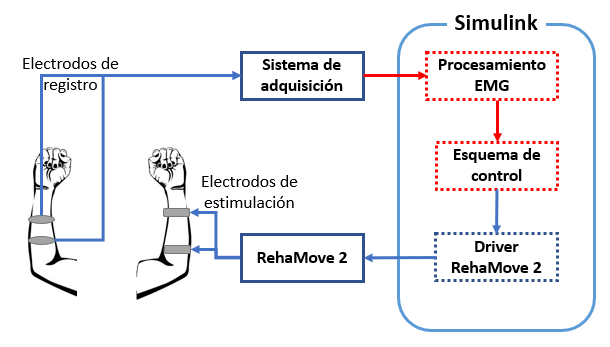
\includegraphics[scale=0.7]{SistemaPropuesto.png}
	\caption[Sistema propuesto para el proyecto]{Sistema propuesto para el proyecto. Líneas continuas representan entes de hardwares y líneas discontinuas representan entes de software. Elementos en rojo representan zonas de trabajo del proyecto.}
	\label{Figura: SistProp}
\end{figure}


\section{Adquisición de datos en Simulink}
Se utilizó el sistema Cyton Board, el cual tiene una frecuencia de muestreo de 250 Hz, para realizar la adquisición de las señales de sEMG. Dicho sistema utiliza un chip ADS1299 (Texas Instruments Inc., Dallas, E.U.A.) para realizar la conversión analógico-digital de las señales, el cual codifica los datos de cada muestra, utilizando complemento a 2, en un flujo de datos de 27 bytes esquematizado en la Figura \ref{Figura: BusOut}.

%Stream datos ADS
\begin{figure}[htbp]
\centering
	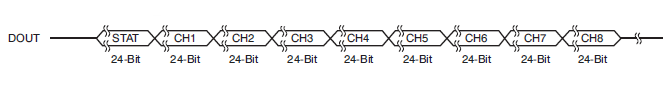
\includegraphics[scale=0.8]{Bus_Dat_Out_ADS.png}
	\caption{Flujo de datos de salida del ADS1299.}
	\label{Figura: BusOut}
\end{figure}

Para realizar la decodificación del flujo de datos dentro de Simulink, se diseñó un subsistema encargado de la solicitud y decodificación de datos, para esto se utilizó el bloque \emph{Query Instrument} del \emph{Instrument Control Toolbox} para realizar la solicitud de datos, los cuales fueron decodificados con bloques de la librería estándar de Simulink. La figura \ref{Figura: DecoSimuT} muestra la implementación dentro de Simulink del sistema antes mencionado.

\hfill \break

%Sistema Simulink
\begin{figure}[htbp]
	\centering
	\begin{subfigure}[htbp]{0.8\textwidth}
		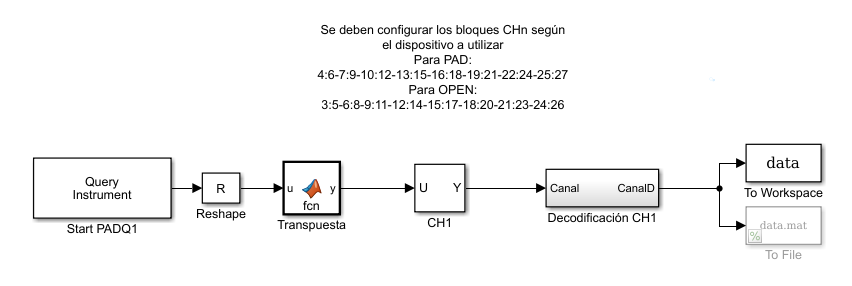
\includegraphics[width=\textwidth]{Read_Simu.png}
		\caption{Vista general del subsistema diseñado para realizar adquisición y decodificación del flujo de datos.}
		\label{Figura: readSimu}
	\end{subfigure}
	\begin{subfigure}[htbp]{0.8\textwidth}
		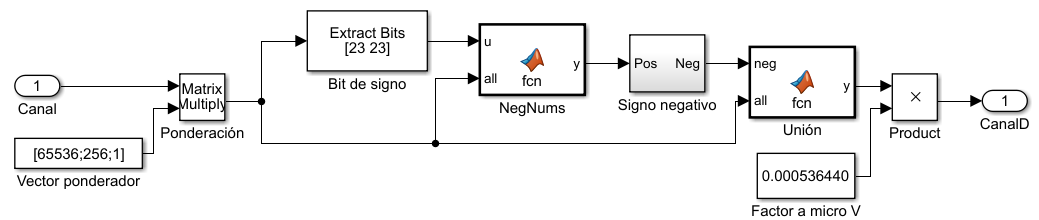
\includegraphics[width=\textwidth]{Deco_Simu.png}
		\caption{Vista interna del subsistema encargado de la decodificación del flujo de datos.}
		\label{Figura: decoSimu}
	\end{subfigure}
	\caption[Subsistema decodificador del flujo de datos]{Subsistema decodificador del flujo de datos implementado en Simulink.}
	\label{Figura: DecoSimuT}
\end{figure}

\newpage
El funcionamiento del subsistema responsable de la solicitud y decodificación de datos implementado dentro de Simulink se encuentra esquematizado en la Figura \ref{Figura: DecoStream}, y lleva a cabo el siguiente algoritmo:

\begin{enumerate}
	\item Se realiza la adquisición de N muestras, lo cual generará un vector columna con dimensión $\mathbb{R}^{27*N\times 1}$ (Figura \ref{Figura: DecoStream} \emph{(a)}).
	\item Se aplicar un reshape a dicho vector para obtener una matriz con dimensión $\mathbb{R}^{27\times N}$ (Figura \ref{Figura: DecoStream} \emph{(b)}).
	\item Se obtiene la transpuesta de dicha matriz para obtener una matriz con dimension $\mathbb{R}^{N\times 27}$ (Figura \ref{Figura: DecoStream} \emph{(c)}).
	\item Se realiza la extracción de las columnas asociadas al canal a procesar, obteniendo una matriz con dimensión $\mathbb{R}^{N\times 3}$ (Figura \ref{Figura: DecoStream} \emph{(d)}).
	\item Se realiza el producto matricial de la matriz del canal a procesar con un vector ponderador que contiene el peso de cada columna (byte) para el valor de la muestra de 24 bits (Figura \ref{Figura: DecoStream} \emph{(e)}). El vector ponderador está compuesto por los valores $2^{16}$, $2^8$, $1$. Como resultado de dicho producto se obtiene un vector de dimensión $\mathbb{R}^{N\times 1}$ (Figura \ref{Figura: DecoStream} \emph{(f)}).
	\item Se extraen del vector anterior las muestras en las que se encuentren codificados, en complemento a 2, un número negativo. Esto se realiza al obtener el valor del bit 23 (bit más significativo), y si dicho bit tiene un valor de 1 implica que dicha muestra codifica un número negativo (Figura \ref{Figura: DecoStream} \emph{(g)}).
	\item Se obtiene el complemento a 1 de cada muestra del vector \emph{g}, se suma 1 a cada muestra y se multiplica cada muestra por -1. De esta operación se obtiene un vector con las muestras decodificadas a número negativos (Figura \ref{Figura: DecoStream} \emph{(h)}).
	\item Se insertan los elementos del vector \emph{h} en sus posiciones originales del vector \emph{f}. De este último paso se obtiene un vector con las N muestras decodificadas a números de 24 bits con signo (Figura \ref{Figura: DecoStream} \emph{(i)}).
\end{enumerate}

%Funcionamiento decodificación
\begin{figure}[htbp]
\centering
	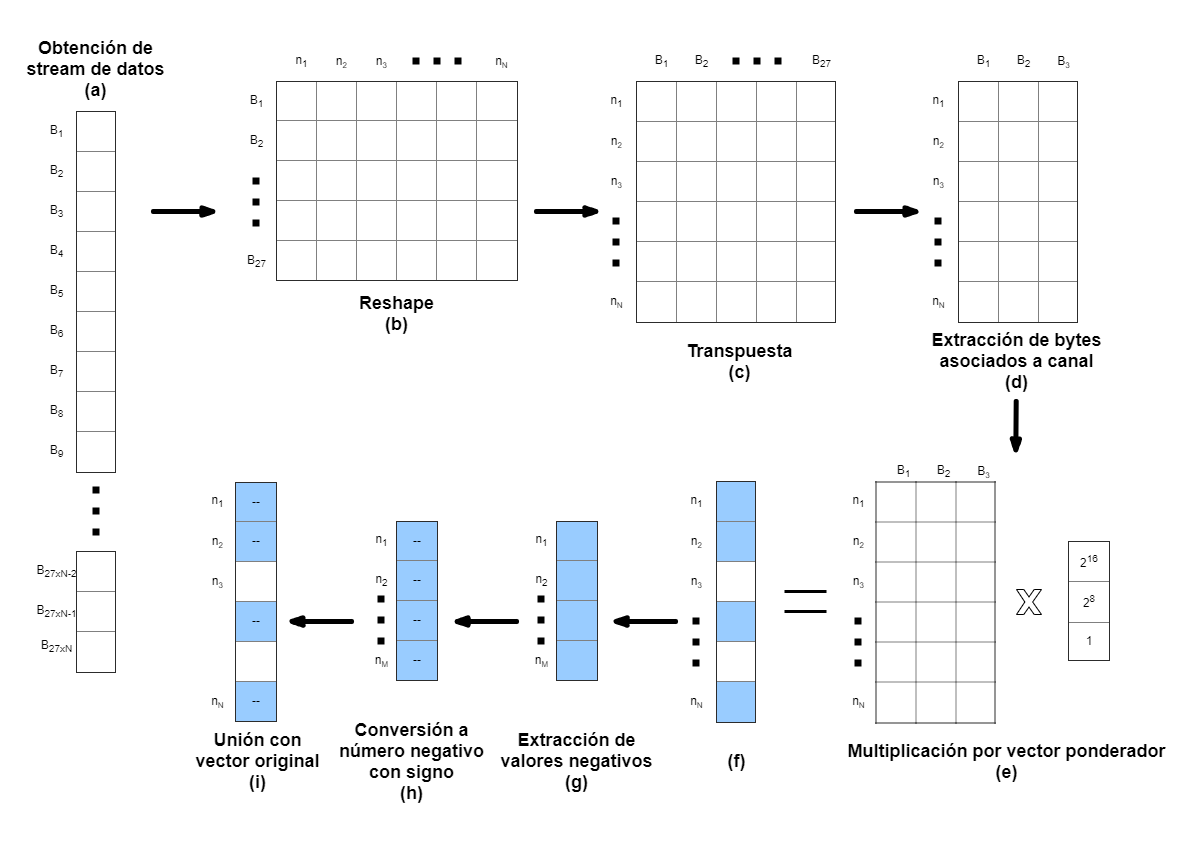
\includegraphics[width=\textwidth]{DecoStream.png}
	\caption{Funcionamiento del subsistema decodificador del flujo de datos.}
	\label{Figura: DecoStream}
\end{figure}


\newpage
\section{Evaluación de bloque de adquisición y decodificación}
Se llevó a cabo un procedimiento para evaluar el desempeño del subsistema diseñado en Simulink para la adquisición y decodificación de datos. En MATLAB se generó un banco de señales senoidales conformado por 5 senoidales puras de 1 Hz, 5 Hz, 10 Hz, 20 Hz y 50 Hz (\ref{Figura: SenPur}), dos senoidales de 50 Hz moduladas en amplitud con una envolvente de una recta con pendiente negativa (\ref{Figura: LinAte}) y una exponencial decreciente (\ref{Figura: ExpAte}), y una senoidal de 50 Hz modulada en amplitud con una envolvente que simula la señal sEMG correspondiente a la tarea de incrementar gradualmente una contracción muscular, mantener dicha contracción y relajar el músculo gradualmente (\ref{Figura: Contra}). Todas las señales del banco se diseñaron con una frecuencia de muestreo de 250 Hz y una duración de 5 segundos, excepto la última, que se diseñó con una duración de 15 segundos; adicionalmente, todas las señales se generaron como objetos de audio dentro de MATLAB, para poder reproducirlas como audio y a partir de la salida de audio de la computadora poder acceder a ellas.

%Figura de senoidales MATLAB
\begin{figure}[htbp]
	\centering
	\begin{subfigure}[htbp]{0.5\textwidth}
		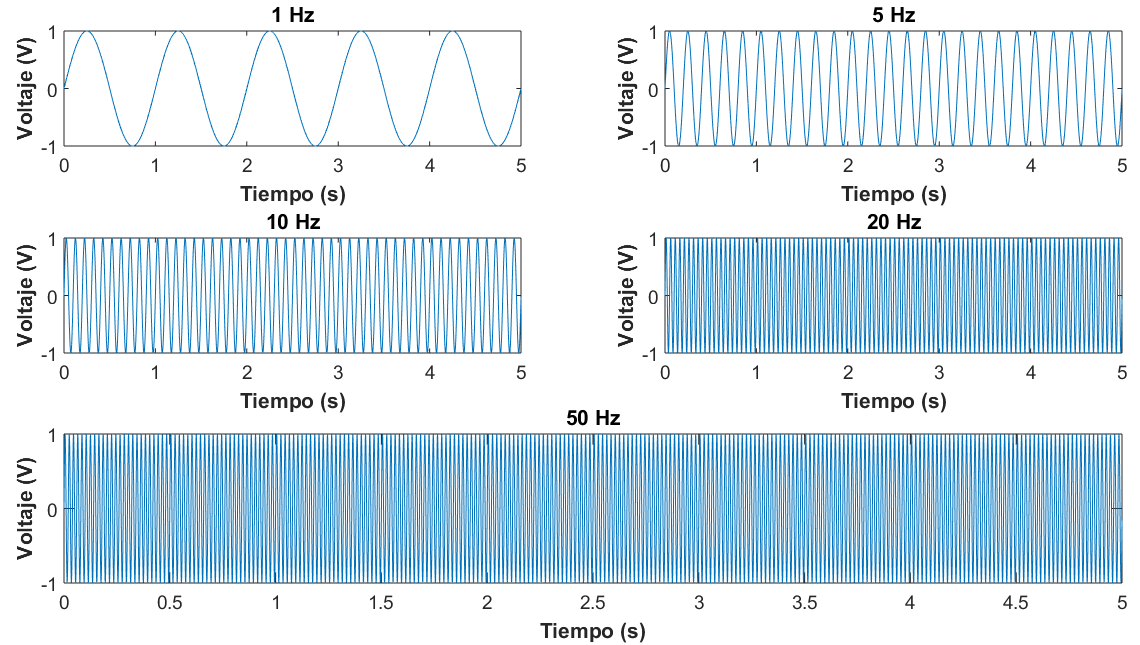
\includegraphics[width=\textwidth]{Sen_Pur.png}
		\caption{Senoidales puras a diferentes frecuencias.}
		\label{Figura: SenPur}
	\end{subfigure}
	\hfill
	\begin{subfigure}[htbp]{0.4	\textwidth}
		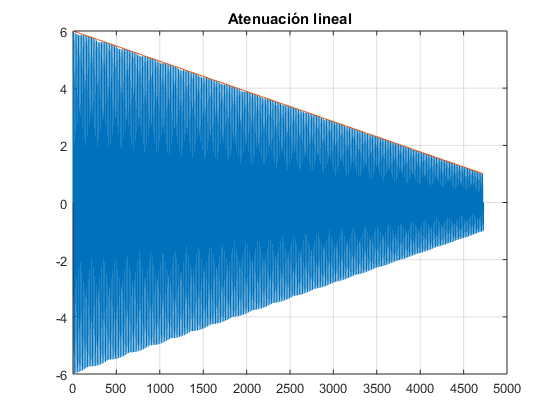
\includegraphics[width=\textwidth]{Lin_Ate.png}
		\caption{Senoidal de 50 Hz con atenuación lineal.}
		\label{Figura: LinAte}
	\end{subfigure}
	\hfill
	\begin{subfigure}[htbp]{0.4\textwidth}
		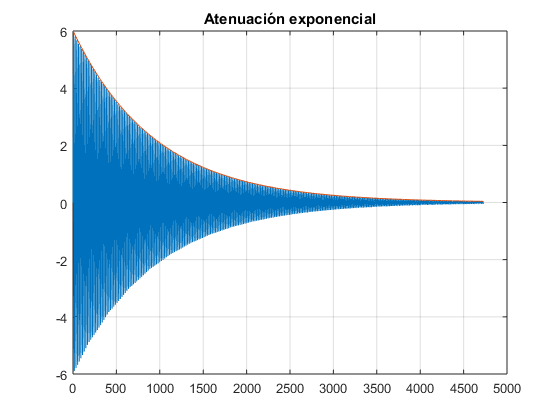
\includegraphics[width=\textwidth]{Exp_Ate.png}
		\caption{Senoidal de 50 Hz con atenuación exponencial.}
		\label{Figura: ExpAte}
	\end{subfigure}
	\hfill
	\begin{subfigure}[htbp]{0.4\textwidth}
		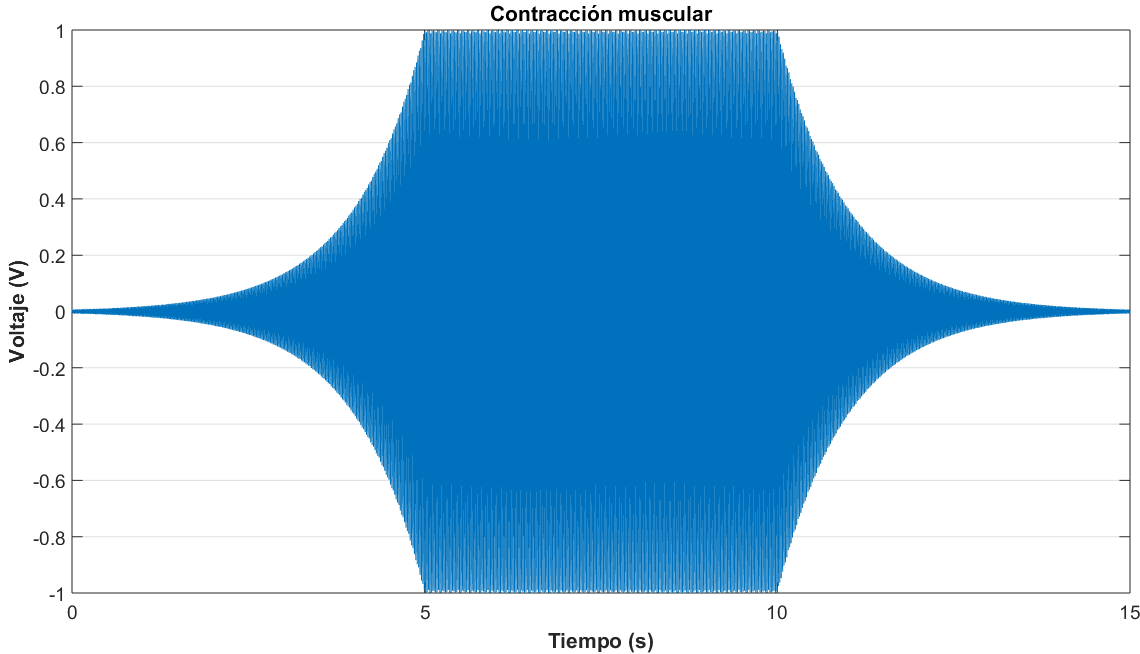
\includegraphics[width=\textwidth]{Contra.png}
		\caption{Senoidal de 50 Hz simulando el sEMG de una contracción muscular.}
		\label{Figura: Contra}
	\end{subfigure}	
	\caption{Banco de señales para evaluación de adquisición.}
	\label{Figura: SenalesEva}
\end{figure}

\newpage
El proceso para la evaluación del funcionamiento del subsistema de adquisición se llevó a cabo de la siguiente manera:
\begin{enumerate}
	\item Se realiza la adquisición de tres tantos de todas las señales del banco de señales de prueba.
	\begin{enumerate}
		\item Se conecta una punta de un jack de audio de 3.5 mm (Figura NUM) a la salida de audio de la computadora. La otra punta se conectó al dispositivo de adquisición (Cyton Board) de la siguiente forma: los pines \emph{izquierdo} y \emph{derecho} se conectaron a la entrada diferencial, mientras que el pin \emph{tierra} se conectó a la entrada BIAS.
		\item Se realiza la solicitud de datos utilizando el subsistema decodificador implementado en Simulink, y al mismo tiempo se inicia el conteo de un cronómetro.
		\item Tras haber transcurrido 2 s en el cronómetro, se procede a reproducir la señal de audio de prueba.
		\item Tras haber transcurrido 10 s (20 s para la simulación del sEMG de una contracción), se detiene la adquisición del subsistema de Simulink y se guardan los datos de adquisición dentro de un archivo con extensión \emph{.mat}.
	\end{enumerate}
	\item Se cargan, dentro del workspace de MATLAB, los datos de las señales adquiridas y los datos de las señales patrón.
	\item Se procede a calcular el coeficiente de correlación de Pearson (Ecuación \ref{Ecu: CorrePea}) entre las señales adquiridas y su correspondiente señal patrón.
	\item Se obtiene la media aritmética de todos los valores obtenidos al aplicar el coeficiente de correlación de Pearson. El valor obtenido se utiliza como indicador de la calidad del subsistema de adquisición y decodificación de datos.
\end{enumerate}

%Ecuación correlación Pearson
\begin{equation}
	r = \frac{\sigma_{xy}}{\sigma_{x}\sigma_{y}}
	\label{Ecu: CorrePea}
\end{equation}


\section{Protocolo para registro de sEMG}
Para garantizar una repetibilidad en los registros de sEMG se implementó un protocolo para realizar la adquisición de dicha señal. Dicho protocolo tiene las caracteristicas mostradas a continuación:

\begin{itemize}
	\item Frecuencia de muestro de sistema de adquisición: 250 Hz.
	\item Canales 1 y 2 para realizar adquisición.
	\item Electrodos: Covidien H124SG
	\item Canal 1: Digitorum flexor
	\begin{itemize}
		\item Medir antebrazo de lado ventral de codo a muñeca.
		\item Palpar músculo al 30\% de la medida obtenida.
		\item Colocar dos electrodos separados 2 cm (Figura \ref{Figura: E_Cie}).
	\end{itemize}
	\item Canal 2: Digitorum extensor
	\begin{itemize}
		\item Medir antebrazo de lado dorsal de codo a muñeca.
		\item Palpar músculo al 50\% de la medida obtenida.
		\item Colocar dos electrodos separados 2 cm (Figura \ref{Figura: E_Ape}).
	\end{itemize}
	\item Referencia: Colocar electrodo en codo.
\end{itemize}

\begin{figure}[htbp]
	\centering
	\begin{subfigure}[htbp]{0.3\textwidth}
		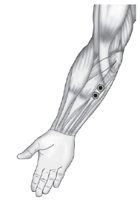
\includegraphics[width=\textwidth]{E_Cie.png}
		\caption{Ubicación de electrodos para digitorum flexor.}
		\label{Figura: E_Cie}
	\end{subfigure}
	\hfill
	\begin{subfigure}[htbp]{0.3\textwidth}
		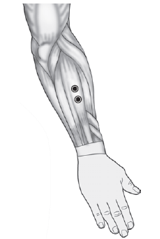
\includegraphics[width=\textwidth]{E_Ape.png}
		\caption{Ubicación de electrodos para digitorum extensor.}
		\label{Figura: E_Ape}
	\end{subfigure}
	\caption[Posicionamiento de electrodos para registro de sEMG]{Posicionamiento de electrodos para realizar registros de sEMG. Recuperado de \cite{Cavalcanti-Garcia2009}.}
	\label{Figura: E_sEMG}
\end{figure}

\section{Procesamiento de sEMG}

Se diseñaron tres filtros Butterworth para realizar el procesamiento de sEMG: un filtro pasa altas con frecuencia de corte de 15 Hz,para eliminar las variaciones en la línea base del registro; un filtro pasa bajas con frecuencia de corte de 100 Hz, para eliminar armónicos de 60 Hz y demás interferencias de alta frecuencia; y un filtro rechaza banda centrado en 60 Hz, para reducir la interferencia de la línea. Las gráficas de respuesta en frecuencia de estos filtros se muestran en las Figuras \ref{Figura: FiltroPA} a \ref{Figura: FiltroRB}.

\begin{figure}[htbp]
	\centering
	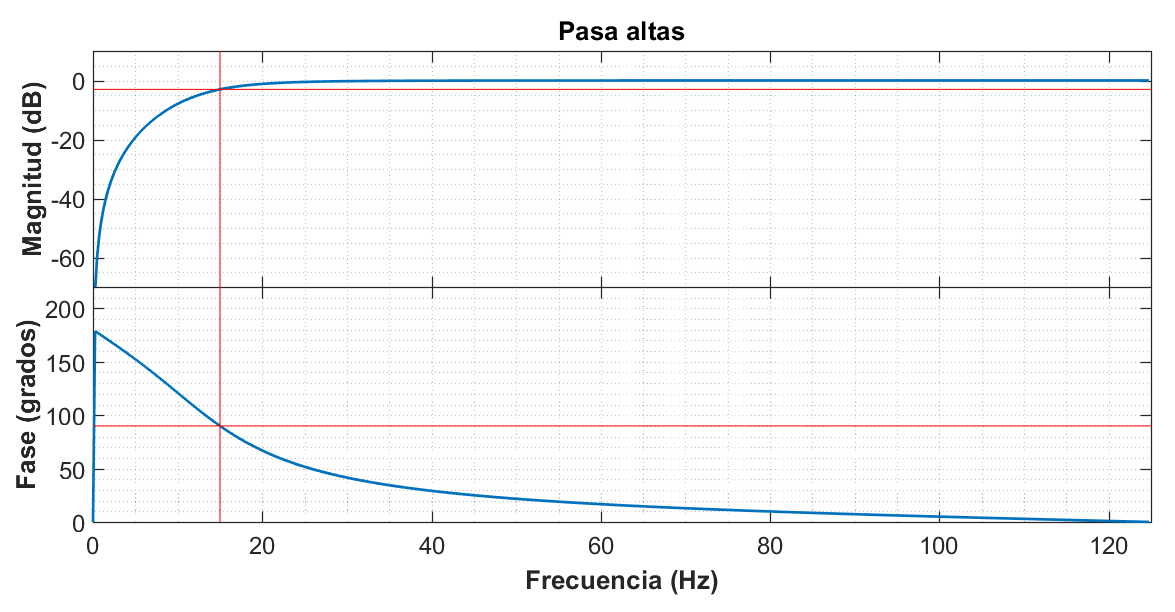
\includegraphics[width=0.7\textwidth]{FiltroPA15Hz_PADQ.png}
	\caption{Filtro pasa altas para conseguir línea base estable.}
	\label{Figura: FiltroPA}
	
	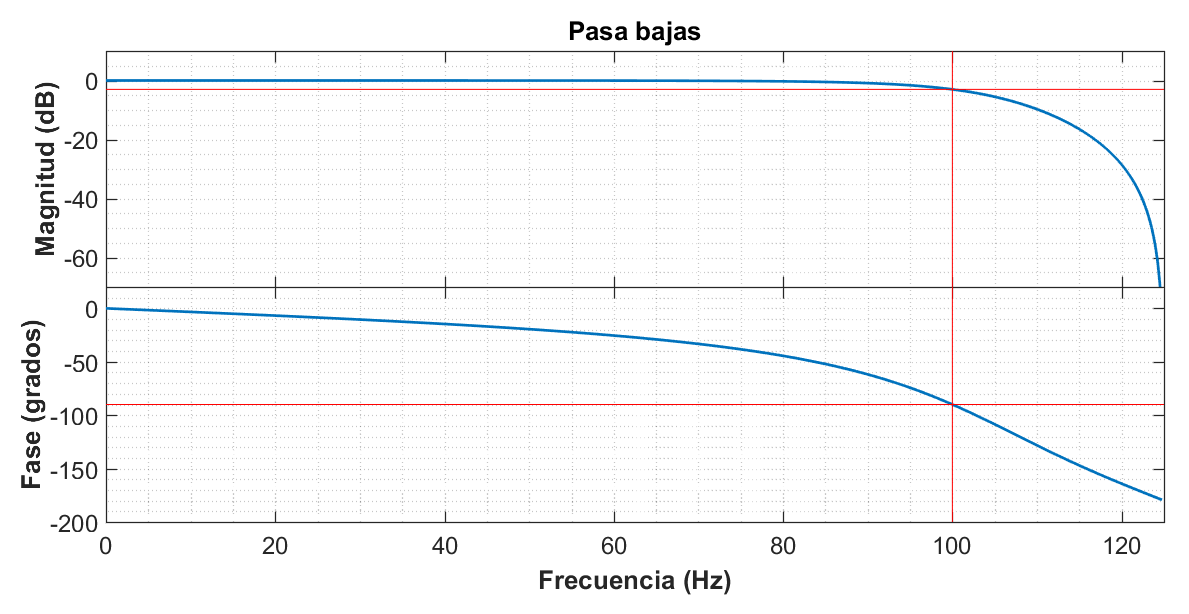
\includegraphics[width=0.7\textwidth]{FiltroPB100Hz_PADQ.png}
	\caption{Filtro pasa bajas para eliminar interferencias de alta frecuencia y armónicos de 60 Hz.} 
	\label{Figura: FiltroPB}
	
	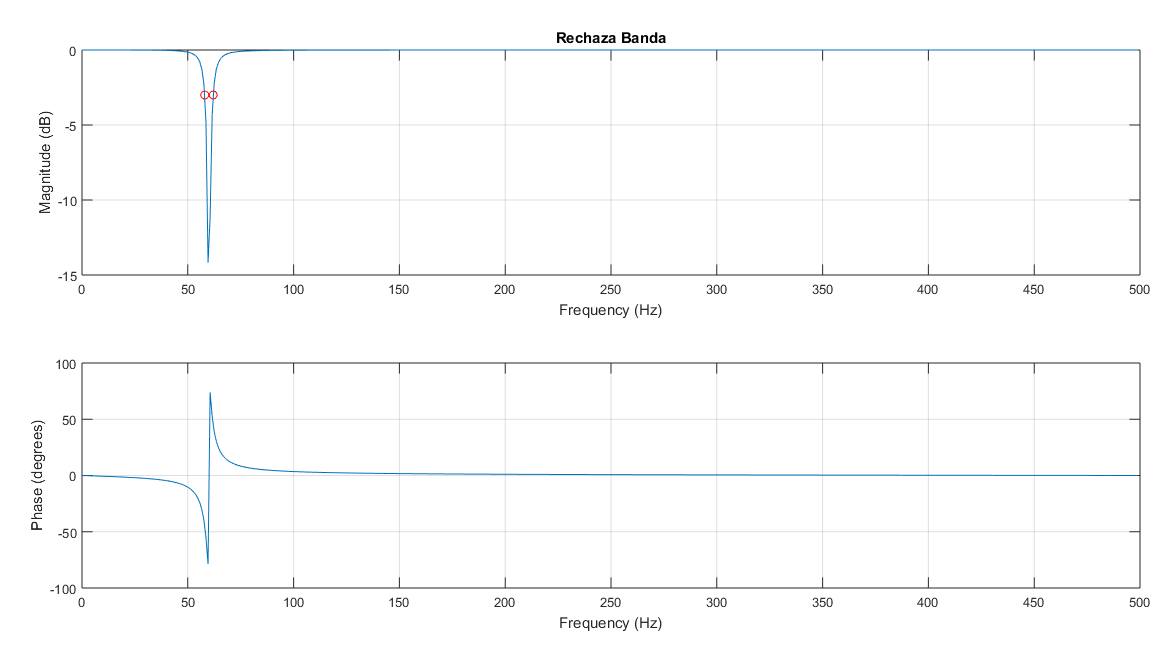
\includegraphics[width=0.7\textwidth]{FiltroRB_58_62_PADQ.png}
	\caption{Filtro rechaza banda para reducir interferencia de 60 Hz.}
	\label{Figura: FiltroRB}
\end{figure}

Se implementó dentro de Simulink un bloque responsable de obtener el valor RMS de ventanas de registro de 100 ms de sEMG para utilizar dicho descriptor de amplitud como señal de control. Adicionalmente se implementó un filtro de de mediana de 10 muestras (Ecuación \ref{Ecu: Mediana}), el cual tiene como propósito conseguir una señal de RMS suavizada

%Ecuación filtro mediana
\begin{equation}
	y[n] = mediana(x[n]:x[n-N])
	\label{Ecu: Mediana}
\end{equation}

\newpage
\section{Esquema de control}
Se diseñó un sistema basado en una combinación de máquina de estados finitos con un control lineal. El sistema requiere de un proceso de calibración previa donde se obtienen 8 umbrales tras la repetición de 4 movimientos, dos umbrales corresponden a los valores RMS promedio de los dos canales de adquisición a lo largo de la tarea \emph{cierre de mano ligero}, otros dos corresponden a los valores RMS promedio de la tarea \emph{cierre de mano completo}, mientras que los 4 restantes corresponden a los valores RMS promedio de las tareas \emph{apertura de mano ligera} y \emph{apertura de mano completa}. Además, tras la calibración se obtiene también un factor denominado \emph{detector de movimiento}, el cual se obtiene tras calcular la diferencia promedio entre los canales de adquisición a lo largo de la tarea de apertura de mano. Adicionalmente se realiza una calibración de la estimulación eléctrica, la cual utiliza el sistema de colocación de electrodos de estimulación descrito en \cite{AnaMartin2019}, donde se obtiene los valores en amplitud de los umbrales motores y funcionales de las tareas de apertura y cierre de mano.

El detector de movimiento se utiliza para realizar el control por máquina de estados finitos (Figura \ref{Figura: FSM_control}), la cual consisten en determinar si la diferencia de amplitudes entre canales ha pasado el valor del detector de movimiento, si es así, el control prosigue con la tarea de apertura de mano, en caso contrario, el control procede a la tarea de cierre de mano.

\begin{figure}[htbp]
	\centering
	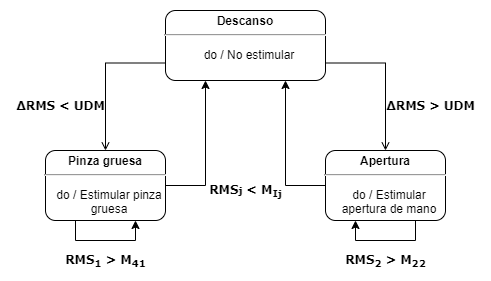
\includegraphics[scale=0.9]{FSM_Control.png}
	\caption{Máquina de estados finitos encargada de la detección de movimiento e inicio del control lineal.}
	\label{Figura: FSM_Control}
\end{figure}

Dentro del control de cada tarea, se utilizan los umbrales de las tareas ligeras para realizar la activación del control lineal, el cual modula la amplitud de la corriente eléctrica, del canal asociado al movimiento detectado, utilizando la recta descrita por la Ecuación \ref{Ecu: Mapeo}, donde $A$ representa la amplitud que inyectará el estimulador eléctrico, $A_{max}$ es el umbral funcional de estimulación eléctica, $A_{min}$ es el umbral motor de estimulación eléctica, $D$ representa el valor RMS actual, mientras que $D_{max}$ y $D_{min}$ representan los umbrales RMS de la tarea completa y ligera del canal asociado al movimiento detectado (canal 1 para cierre de mano y canal 2 para apertura de mano). Adicionalmente se aplica la función máximo entero a la recta debido a que el dispositivo de estimulación eléctrica sólo admite valores enteros, y también se aplica un criterio de saturación de corriente eléctrica para evitar que tras una contracción muscular muy fuerte se genere un valor de amplitud de corriente eléctrica dañino para el sujeto.

%Ecuación mapeo lineal
\begin{equation}
	A = \frac{A_{max} - A_{min}}{D_{max} - D_{min}}(D - D_{min}) + A_{min}
	\label{Ecu: Mapeo}
\end{equation}

%\section{Tarea objetivo}
%{\color{red}INCLUIR TAREA OBJETIVO DE ENTRENAMIENTO CON TRAPEZOIDAL EN LÍNEA}
